\chapter{Benchmarks}


\section{TREC evaluation}

\paragraph{}
To assess the system's performance, we utilized the TREC Eval tool, which was created by the Text REtrieval Conference (TREC) to establish a standardized method for comparing the efficacy of various search engines.

TREC Eval accepts a collection of search outcomes and relevant documents as input, subsequently employing several evaluation metrics to gauge the search result quality. These metrics encompass reciprocal rank, alongside more sophisticated measures such as mean average precision (MAP) and normalized discounted cumulative gain (NDCG).

\paragraph{Results}
The following table \ref{tab:metric_comparison} makes comparisons of our engine's performance with other search engines freely available, we used the  \href{https://msmarco.blob.core.windows.net/msmarcoranking/msmarco-test2020-queries.tsv.gz}{\texttt{msmarco-test2020-queries}} and set those engines to retrieve the first twenty results for each query.

\begin{table}[H]
	\centering
	\begin{tabular}{|l|>{\ttfamily}r|>{\ttfamily}r|>{\ttfamily}r|}
		\hline
		Metric & \normalfont\textbf{SEPP} & \normalfont\textbf{Anserini} & \normalfont\textbf{Chang's} \\
		\hline
		mAP & 0.1982 & 0.1942 & 0.0794 \\
		RR & 0.8110 & 0.8215 & 0.7285 \\
		ndcg & 0.3376 & 0.3364 & 0.1681\\
		ndcg@10 & 0.4750 & 0.4876 & 0.4075 \\
		ndcg@20 & 0.4705 & 0.4705 & - \\
		set P & 0.4815 & 0.4667  & 0.5163 \\
		set R & 0.2600 & 0.2496 & 0.0987 \\
		set F & 0.2781 & 0.2670 & 0.1437 \\
		\hline
	\end{tabular}
	\caption{comparison of our project and Anserini's}
	\label{tab:metric_comparison}
\end{table}

\section{Time statistics}

\paragraph{}
The table presents the query processing times for the provided collection. 

Furthermore, we have included a histogram illustrating the distribution of execution times for run queries, comparing two methods: BMM and DAAT. This graphical representation allows for a visual comparison of the execution time distribution between the two query processing approaches.

\subsection{Queries' execution times}
	\begin{table}[h]
		\centering
		\begin{tabular}{|l|>{\ttfamily}r|>{\ttfamily}r|>{\ttfamily}r|}
			\hline
			Algorithm & \normalfont\textbf{AVG [ms]} & \normalfont\textbf{STD DEV [ms]} & \normalfont\textbf{MAX [ms]} \\
			\hline
			DAAT & 25.88 & 19.69 & 78.68 \\
			BMM & 6.67 & 6.29 & 42.48 \\
			\hline
		\end{tabular}
		\caption{Execution times in milliseconds for different algorithms}
		\label{tab:algorithm_times}
	\end{table}
	
	\begin{figure}[H]
		\centering
		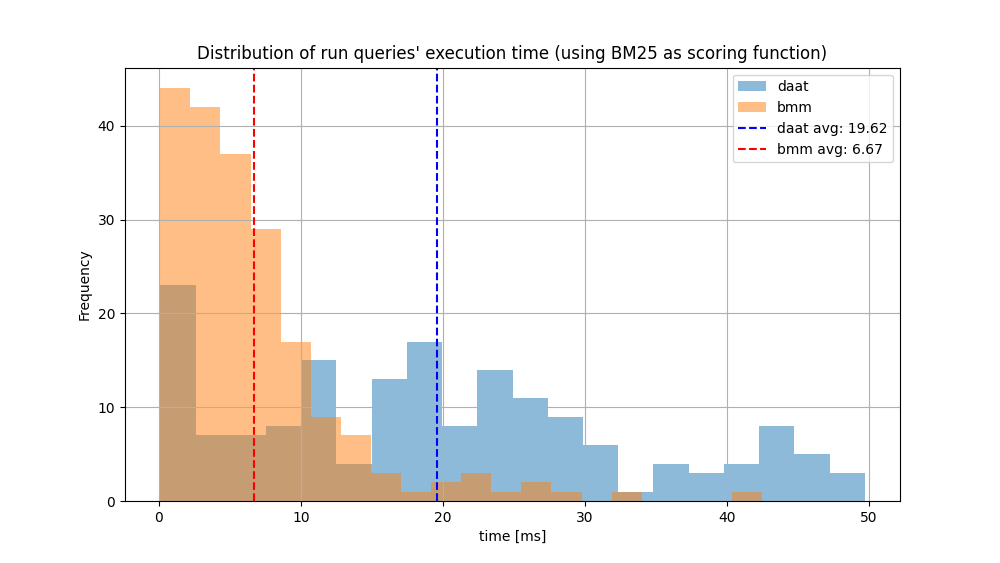
\includegraphics[width=1\textwidth]{assets/times_distrib.png}
		\caption{Distribution of times}
		\label{fig:time_distribution}
	\end{figure}
	
\subsection{Index's construction time}
\lstinputlisting[caption={Indexing program's output: it takes less than 1 minute and 20 seconds to build it}, label={lst:example_output}]{assets/build time.txt}
	
\section{Files' size}

\paragraph{}
The following table shows the file sizes presented in megabytes, divided int the indices' main files: Document Index, Local Lexicon, and Posting List.

\begin{table}[H]
	\centering
	\begin{tabular}{|l|*{5}{c|}c|}
		\hline
		& \textbf{Partition 0} & \textbf{Partition 1} & \textbf{Partition 2} & \textbf{Partition 3} & \textbf{Partition 4} & \textbf{Total} \\
		\hline
		Document Index & 46 & 47 & 46 & 46 & 17 & \textbf{202} \\
		Local Lexicon & 22 & 23 & 23 & 23 & 12 & \textbf{103} \\
		Posting Lists & 131.5 & 174.5 & 174.5 & 173.5 & 61.7 & \textbf{715.7} \\
		\hline
		\multicolumn{6}{|c|}{Global Lexicon} & \textbf{14} \\
		\hline
		\multicolumn{6}{|c|}{\textbf{TOTAL}} & \textbf{1034.7} \\
		\hline
	\end{tabular}
	\caption{Files' sizes, figures in megabytes}
	\label{tab:spanning_table}
\end{table}

\paragraph{}
To provide a clearer visualization, we have included a tree diagram below where the files' structure is depicted.

\lstinputlisting[caption={Files tree}, label={lst:tree}]{assets/files sizes.txt}


\section{Limitations}
% DAAT non ottimizzato per le query conjunctive
SEPP has some drawbacks. One issue is with our word normalization algorithm, our search engine's use of it doesn't handle synonyms or related terms well. Basically, every word is treated separately, so if your search doesn't exactly match the words in the documents, BM25 might not score them accurately for relevance.

Our search engine's way of breaking down text into smaller bits also has its problems. It just chops off punctuation without thinking, which means we might lose important stuff like acronyms, hashtags, dates, or prices. Plus, it doesn't recognize phrases made up of multiple words. On top of that, SEPP doesn't catch spelling mistakes or different word forms.

\paragraph{Possible solutions}
SEPP's drawbacks include word normalization issues — enhance it for synonyms and related terms. Modify text tokenization to retain punctuation for acronyms, hashtags, and multiword expressions. Implement spell-check and word form recognition for improved flexibility. Utilize NLP, user feedback, and BM25 adjustments for more accurate search outcomes. For example: experiment with BM25 parameters to optimize the search engine's scoring mechanism. Fine-tuning these parameters could improve relevance scoring, even when search queries don't precisely match document words.

